% Presentation for my talk at GopherCon Russia 2020
%
% (c) Alexey Naidyonov 2020
% License CC-BY 3.0
%
\documentclass[
  11pt,aspectratio=1610,pdf,hyperref={unicode,colorlinks=false}
]{beamer}
\usetheme{gophercon}
\usepackage{pgfpages}
\usepackage[1080p]{itoolabs-graphics}

\setbeameroption{hide notes} % Only slides
%\setbeameroption{show only notes} % Only notes
%\setbeameroption{show notes on second screen=right} % Both
\setbeamertemplate{note page}{\pagecolor{yellow!5}\insertnote}

\title{
  TLA+ Tools: \\ 
  практичный инструмент \\ 
  формальной верификации алгоритмов
}
\subtitle{
  (или что ещё разработчику на Golang точно\\надо изучить во время карантина)
}
\institute[\href{https://itoolabs.com}{itoolabs.com}]{%
  \href{https://itoolabs.com}{ITooLabs}}
\author[\href{https://twitter.com/growler}{@growler}]{%
  \href{https://twitter.com/growler}{Alexey Naidyonov}}
\event{\href{https://www.gophercon-russia.ru}{GopherCon Russia 2020}}
\date[28.03.2020]{Mar 28 2020}
\eventlogo{
\includegraphics[keepaspectratio,width=.15\paperwidth]{gophercon-logo.png}}

\begin{document}

\begin{frame}[plain]\titlepage\end{frame}

% Что такое программа?
\begin{frame}
  \centering\Large\bf{Что такое программа?}
\end{frame}

% Ответ на вопрос
\begin{frame}[c,fragile]
  \begin{columns}
    \begin{column}{.05\textwidth}\end{column}
    \begin{column}{.3\textwidth}
      \begin{code}[fontsize=\large]{go}
        var i = 0
        for i < 3 {
          i = i + 1
        }
      \end{code}
    \end{column}
    \begin{column}{.3\textwidth}
      \centering
      \onslide<2->{\resizebox{!}{.8\textheight}{%
        \begin{tikzpicture}[node distance = 3cm, auto, font=\ttfamily]
          \tikzstyle{decision} = [diamond, draw, text width=4.5em, text badly centered, inner sep=0pt]
          \tikzstyle{block} = [rectangle, draw, text width=5em, text centered, rounded corners, minimum height=4em]
          \tikzstyle{line} = [draw, -latex]
	        \node [block] (init) {i = 0};
	        \node [decision, below of=init] (loop) {i < 3};
	        \node [block, below of=loop] (eval) {i = i + 1};
	        \path [line] (init) -- (loop);
	        \path [line] (loop) -- node [near start] {Yes} (eval);
	        \path [line] (eval.west) |- ([xshift=-2cm]eval.center) -- ([xshift=-2cm]loop.center) -- (loop);
	        \path [line] (loop.east) -- node [near start] {No} ([xshift=2cm]loop.east);
        \end{tikzpicture}
        }
      }    
    \end{column}
    \begin{column}{.3\textwidth}
      \centering
      \onslide<3>{\resizebox{!}{.8\textheight}{%
        \begin{tikzpicture}[->,>=stealth',node distance = 1cm, auto]
          \tikzstyle{every state}=[ellipse,font=\ttfamily]
          \node[state] (A)              {i = 0};
          \node[state] (B) [below=of A] {i = 1};
          \node[state] (C) [below=of B] {i = 2};
          \node[state] (D) [below=of C] {i = 3};
          \path (A) edge (B) (B) edge (C) (C) edge (D);
        \end{tikzpicture}
        }
      }
    \end{column}
    \begin{column}{.05\textwidth}\end{column}
  \end{columns}
\end{frame}

% Пример с двумя агентами
\begin{frame}[c,fragile]
  \begin{columns}
  \begin{column}{.2\textwidth}\end{column}
  \begin{column}{.3\textwidth}
    {\Large\bf Process 1}
    \par\vspace{2ex}
    \begin{code}[fontsize=\large]{go}
      a = b + 1
      b = a + 1
    \end{code}
    \par\vspace{5ex}
    {\Large\bf Process 2}
    \par\vspace{2ex}
    \begin{code}[fontsize=\large]{go}
      b = a + 1
      a = b + 1
    \end{code}
  \end{column}
  \begin{column}{.4\textwidth}
  \begin{tikzpicture}[->,>=stealth',node distance=2.5cm and 2cm,semithick,on grid]
    \tikzset{
      state/.style={ellipse,draw,align=left,font=\ttfamily\small},
      edge/.style={->}
    }
    \only<6>{\tikzset{
      state/.prefix style={draw=red}
    }}
    \only<7>{\tikzset{
      edge/.prefix style={draw=blue}
    }}
    \node[state] (A) {a = 0 \\ b = 0};
    \node[left of=A, align=center,red,visible on=<6>] {Состояния\\(states)};
    \node[right of=A, align=center,blue,visible on=<7>] {Пути\\выполнения\\(behaviours)};
    \node[state,visible on={<2-3,6->},label={[visible on={<2-3,6->}]150:p1},align=left] (B) [below left=of A]
      {a = 1\\b = 2};
    \node[state,visible on={<3,6->},label={[visible on={<3,6->}]150:p2},align=left] (C) [below=of B]
      {a = 3\\b = 2};
    \node[state,visible on={<4->},label={[visible on={<4->}]30:p2},align=left] (D) [below right=of A]
      {a = 2\\b = 1};
    \node[state,visible on={<5->},label={[visible on={<5->}]30:p1},align=left] (E) [below=of D]
      {a = 2\\b = 3};
    \path[edge, visible on={<2-3,6->}] (A) edge (B);
    \path[edge, visible on={<3,6->}]   (B) edge (C);
    \path[edge, visible on={<4->}]     (A) edge (D);
    \path[edge, visible on={<5->}]     (D) edge (E);
  \end{tikzpicture}
  \end{column}
  \begin{column}{.2\textwidth}\end{column}
  \end{columns}
\end{frame}

% оценка мощности множества состояний
\begin{frame}[c]
  \Large%
  \begin{gather*}
    (m \cdot n) \frac{(m \cdot n)!}{(n!)^m},
    \intertext{\Large где}
    {\Large \begin{tabular}{>{\(}r<{\)}@{\ -\ }l}
      m & количество процессов \\
      n & длина пути выполнения
    \end{tabular}}
  \end{gather*}
\end{frame}

% пример пространства состояний CAN
\begin{frame}[c]
  \centering
  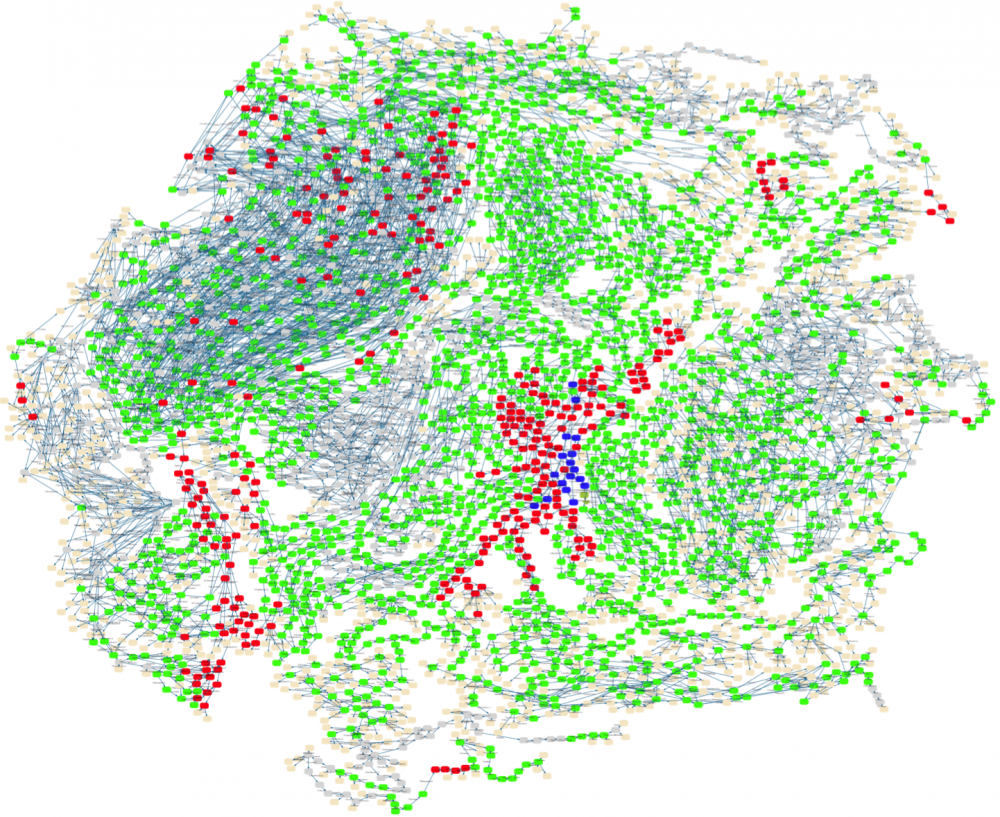
\includegraphics[keepaspectratio, height=.85\textheight]{media/1000px-CANBus_sfdp.png}\\
  {\tiny CAN Bus state space visualization\\[-1\baselineskip]%
  {\color{white!70!black}\url{https://www3.hhu.de/stups/prob/index.php/State_space_visualization_examples}}}
\end{frame}

% штука про отвлечения программиста
\begin{frame}[c]
  \centering
  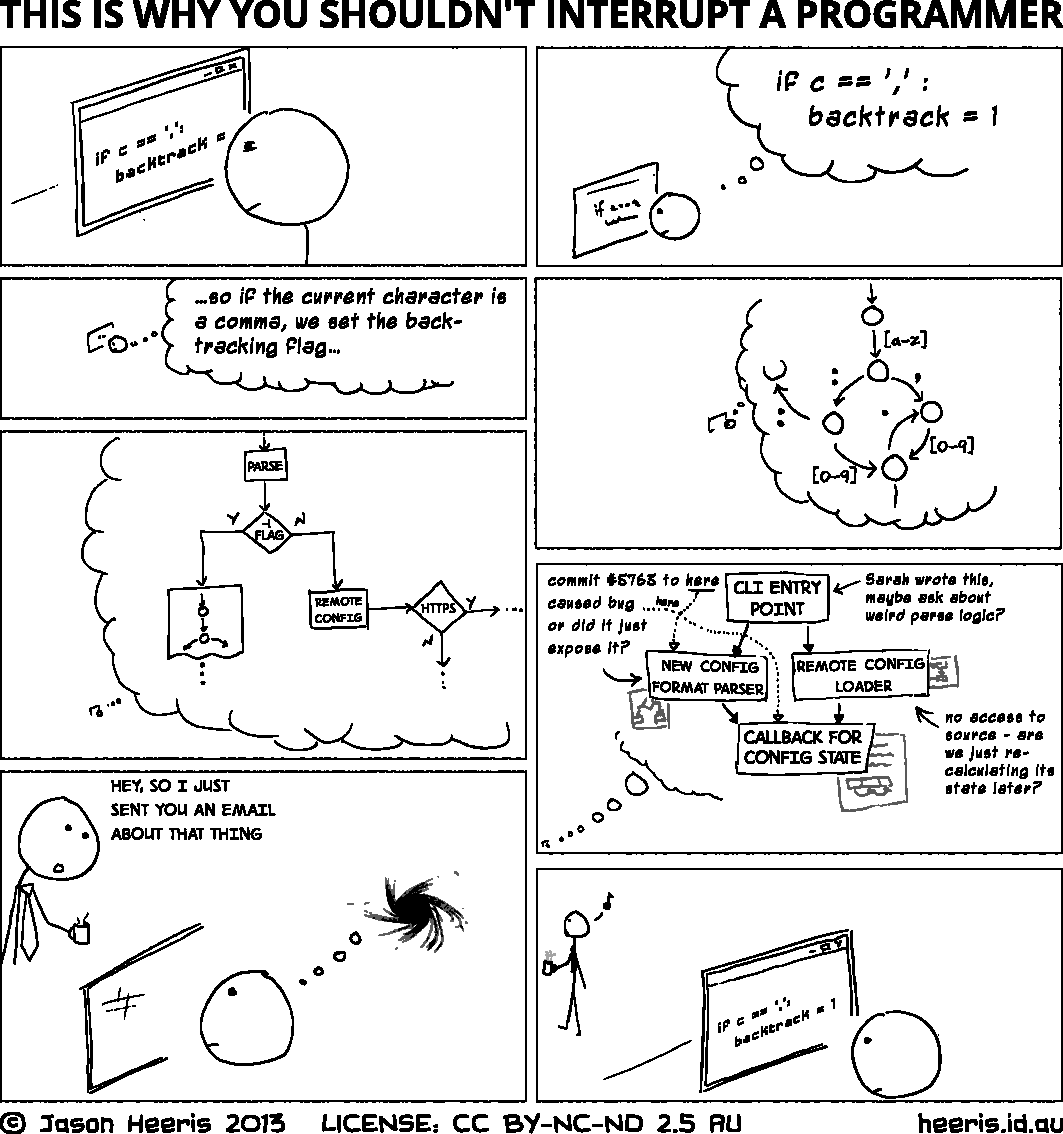
\includegraphics[keepaspectratio, height=.85\textheight]{never-interrupt-programmer.pdf}
\end{frame}

% цитата про распределенные системы
\begin{frame}
  \begin{quote}
    {\Large ``A distributed system is one in which the failure
    of a computer you didn't even know existed can
    render your own computer unusable.''}\\
    \vspace{1ex}
    \hspace*\fill{\small--- Leslie Lamport, May 1987}
  \end{quote}
\end{frame}

% представление Лесли Лэмпорта
\begin{frame}[c]
  \begin{columns}
    \begin{column}{.45\textwidth}      
      {\Large\bf
        Лесли Лэмпорт\\
        (\href{https://lamport.azurewebsites.net}{Leslie Lamport})
      }\\
      \vspace{3ex}
      \large
      \vspace{1ex}
      \begin{itemize}
        \item Lamport timestamps
        \item Bakery algorithm
        \item PAXOS
        \item LaTeX
        \item {\bf TLA+}
      \end{itemize}
    \end{column}
    \begin{column}{.5\textwidth}
      \centering
      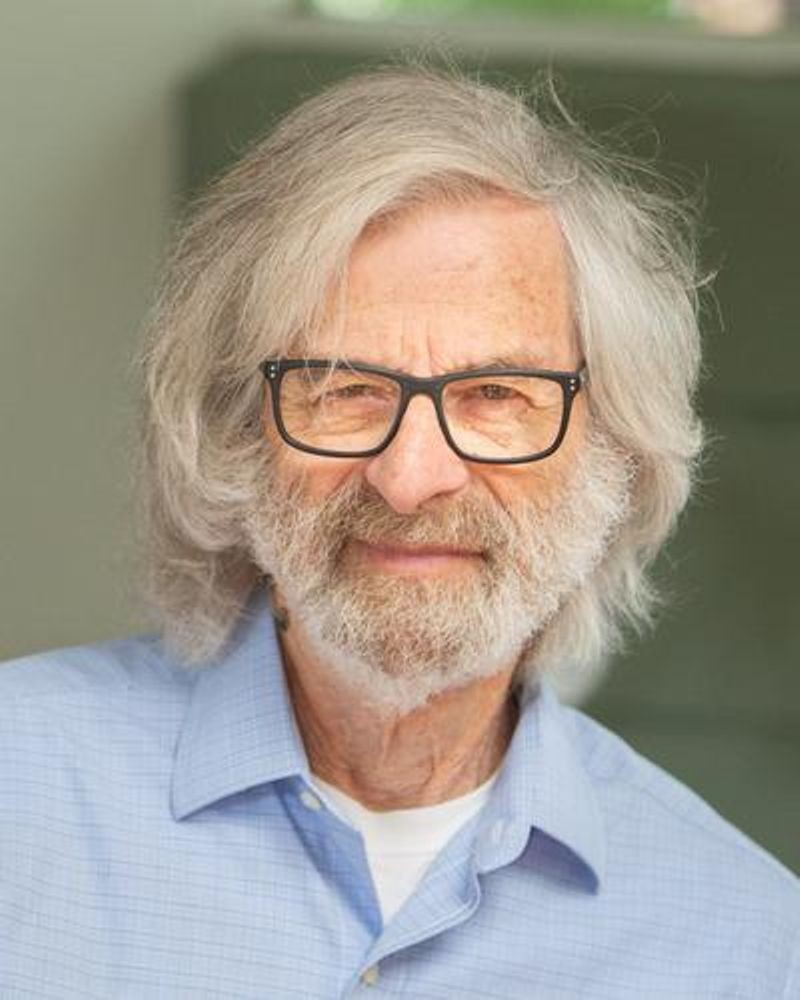
\includegraphics[keepaspectratio, height=.85\textheight]{leslie-lamport.jpg}
    \end{column}
  \end{columns}
\end{frame}  

% TLA+
\begin{frame}[c]  
  \centering\Large\bf
  \href{https://lamport.azurewebsites.net/pubs/lamport-actions.pdf}{Temporal Logic of Actions}
\end{frame}

% что такое TLA+
\begin{frame}[c]
  \centering
  \begin{overlayarea}{.7\textwidth}{.8\textheight}
    \centering\large
    \begin{tabular}{l @{\hspace{3ex}} >{\begin{invisibleenv}<-13>}l<{\end{invisibleenv}} @{\hspace{3ex}} l}
      \multicolumn{3}{c}{\centering\Large\bf\itshape Математическая логика}\pause\\%
      \\%
      \(A \wedge B\) & \Verb|A/\B| & Коньюнкция \pause\\%
      \(A \vee B\)   & \Verb|A\/B| & Дизьюнкция \pause\\%
      \(A \to B\)    & \Verb|A=>B| & Импликация \pause\\%
      \(\neg A\)     & \Verb|~A|   & Отрицание \pause\\%
      \\%
      \multicolumn{3}{c}{\centering\Large\bf\itshape Темпоральная логика}\\%
      \multicolumn{3}{c}{%
        \only<6>{%
          \begin{minipage}{.5\textwidth}%
            \centering\vspace{1.5ex}%
            
\includegraphics[keepaspectratio, height=.35\textheight]{doc-brown.jpg}\\%
            \fontsize{4pt}{1.2}\selectfont\color{white!70!black}\copyright Universal Pictures Amblin Entertainment%
          \end{minipage}%
        }        
      }\pause\\%
      \(\Diamond A\)     & \Verb|<>A|  & Eventually \pause\\%
      \(\Box A\)         & \Verb|[]A|  & Always \pause\\%
      \(A \leadsto B \)  & \Verb|~>A|  & Leads to\pause\\%     
      \(\Box\Diamond A\) \pause & \Verb|[]<>A| & Infinitely often\pause\\%
      \(\Diamond\Box A\) \pause & \Verb|<>[]A| & Eventually always \pause\\%
    \end{tabular}
  \end{overlayarea}
\end{frame}

%
% \begin{tabbing}
% ... line \\
% \hl<1>
% line to be highlighted on slide 1 \\
% \end{tabbing}
%
\def\hl<#1>{%
\alt<#1>{\usebeamercolor[fg]{alerted text}}%
        {\usebeamercolor[fg]{normal text}}%
}

%
% disables topsep for tabbing 
% einvironment 
%
\newenvironment{nstabbing}%
{\setlength{\topsep}{0pt}%
  \setlength{\partopsep}{0pt}%
  \tabbing}%
{\endtabbing}

% пример спецификации счетчика
\begin{frame}[c]
  \begin{columns}
  \begin{column}[c]{.6\textwidth}
    \small
    \moduleLeftDash%
    {\sc module} 00\_Counter    
    \moduleRightDash%
    \hl<2>
    \begin{nstabbing}
      {\sc constants} \= \kill
      {\sc extends}   \> Naturals\\
      [0pt \hl<3>]
      {\sc constants} \> MinValue, MaxValue \\
      [0pt \hl<4>]
      {\sc assume}    \> \( \text{MinValue} < \text{MaxValue} \) \\
      [0pt \hl<5>]
      {\sc variable}  \> counter
    \end{nstabbing}
    \begin{nstabbing}
      \\
      [0pt \hl<6>]
      Invariant \= \( \triangleq \text{counter} \in \text{MinValue}\ldotp\ldotp\text{MaxValue} \) \\
      \\
      [0pt \hl<7>]
      Success \> \( \triangleq \Diamond\Box (\text{counter} = \text{MaxValue}) \)
    \end{nstabbing}    
    \begin{nstabbing}
      Next \= \kill \\
      [0pt \hl<8>]
      Init \> \( \triangleq \text{counter} = \text{MinValue} \) \\
      % \pushtabs \\
      \\
      [0pt \hl<9>]
      Next \> \( \triangleq \text{counter}'= \) \= {\sc if} \( \text{counter} < \text{MaxValue} \) 
      \+ \+ \\      
        {\sc then} counter + 1 \\
        {\sc else} counter \- \- \\
      [0pt \hl<10->]
      Spec \> \( \triangleq \) \= \+ \+ \( \wedge \; \text{Init} \) \\
      [0pt \hl<11->]
        \( \wedge \; \Box[\text{Next}]_\text{counter} \) \\
        [0pt \hl<12>]  
        \( \wedge \; \text{WF}_\text{counter}(\text{Next}) \)
    \end{nstabbing}
    \usebeamercolor[fg]{normal text}
    \bottombar%
  \end{column}
  \begin{column}[c]{.3\textwidth}
    \centering\resizebox{!}{.9\textheight}{
\begin{tikzpicture}[>=latex,line join=bevel,]
  \pgfsetlinewidth{1bp}
%%
\begin{scope}
  \pgfsetstrokecolor{black}
  \definecolor{strokecol}{rgb}{1.0,1.0,1.0};
  \pgfsetstrokecolor{strokecol}
  \draw (8.0bp,8.0bp) -- (8.0bp,276.0bp) -- (146.0bp,276.0bp) -- (146.0bp,8.0bp) -- cycle;
\end{scope}
\begin{scope}
  \pgfsetstrokecolor{black}
  \definecolor{strokecol}{rgb}{1.0,1.0,1.0};
  \pgfsetstrokecolor{strokecol}
  \draw (8.0bp,8.0bp) -- (8.0bp,276.0bp) -- (146.0bp,276.0bp) -- (146.0bp,8.0bp) -- cycle;
\end{scope}
\begin{scope}
  \pgfsetstrokecolor{black}
  \definecolor{strokecol}{rgb}{1.0,1.0,1.0};
  \pgfsetstrokecolor{strokecol}
  \draw (8.0bp,8.0bp) -- (8.0bp,276.0bp) -- (146.0bp,276.0bp) -- (146.0bp,8.0bp) -- cycle;
\end{scope}
\begin{scope}
  \pgfsetstrokecolor{black}
  \definecolor{strokecol}{rgb}{1.0,1.0,1.0};
  \pgfsetstrokecolor{strokecol}
  \draw (8.0bp,8.0bp) -- (8.0bp,276.0bp) -- (146.0bp,276.0bp) -- (146.0bp,8.0bp) -- cycle;
\end{scope}
\begin{scope}
  \pgfsetstrokecolor{black}
  \definecolor{strokecol}{rgb}{1.0,1.0,1.0};
  \pgfsetstrokecolor{strokecol}
  \draw (8.0bp,8.0bp) -- (8.0bp,276.0bp) -- (146.0bp,276.0bp) -- (146.0bp,8.0bp) -- cycle;
\end{scope}
  \pgfsetcolor{black}
  % Edge: -107664775997770560 -> -107664775997770560
  \draw [->,dashed] (104.84bp,262.81bp) .. controls (125.69bp,265.31bp) and (145.0bp,261.04bp)  .. (145.0bp,250.0bp) .. controls (145.0bp,240.77bp) and (131.5bp,236.27bp)  .. (104.84bp,237.19bp);
  % Edge: -107664775997770560 -> -8739362515292856379
  \pgfsetcolor{2}
  \draw [->] (68.0bp,231.83bp) .. controls (68.0bp,224.13bp) and (68.0bp,214.97bp)  .. (68.0bp,196.41bp);
  % Edge: -8739362515292856379 -> -8739362515292856379
  \pgfsetcolor{black}
  \draw [->,dashed] (104.84bp,190.81bp) .. controls (125.69bp,193.31bp) and (145.0bp,189.04bp)  .. (145.0bp,178.0bp) .. controls (145.0bp,168.77bp) and (131.5bp,164.27bp)  .. (104.84bp,165.19bp);
  % Edge: -8739362515292856379 -> 1075403382720062154
  \pgfsetcolor{2}
  \draw [->] (68.0bp,159.83bp) .. controls (68.0bp,152.13bp) and (68.0bp,142.97bp)  .. (68.0bp,124.41bp);
  % Edge: 1075403382720062154 -> 1075403382720062154
  \pgfsetcolor{black}
  \draw [->,dashed] (104.84bp,118.81bp) .. controls (125.69bp,121.31bp) and (145.0bp,117.04bp)  .. (145.0bp,106.0bp) .. controls (145.0bp,96.772bp) and (131.5bp,92.275bp)  .. (104.84bp,93.193bp);
  % Edge: 1075403382720062154 -> 8564275020137105871
  \pgfsetcolor{2}
  \draw [->] (68.0bp,87.831bp) .. controls (68.0bp,80.131bp) and (68.0bp,70.974bp)  .. (68.0bp,52.413bp);
  % Edge: 8564275020137105871 -> 8564275020137105871
  \draw [->,dashed] (104.84bp,46.807bp) .. controls (125.69bp,49.308bp) and (145.0bp,45.039bp)  .. (145.0bp,34.0bp) .. controls (145.0bp,24.772bp) and (131.5bp,20.275bp)  .. (104.84bp,21.193bp);
  % Node: -107664775997770560
\begin{scope}
  \definecolor{strokecol}{rgb}{0.0,0.0,0.0};
  \pgfsetstrokecolor{strokecol}
  \definecolor{fillcol}{rgb}{0.83,0.83,0.83};
  \pgfsetfillcolor{fillcol}
  \filldraw [opacity=1] (68.0bp,250.0bp) ellipse (51.99bp and 18.0bp);
  \draw (68.0bp,250.0bp) node {counter = 0};
\end{scope}
  % Node: -8739362515292856379
\begin{scope}
  \definecolor{strokecol}{rgb}{0.0,0.0,0.0};
  \pgfsetstrokecolor{strokecol}
  \draw (68.0bp,178.0bp) ellipse (51.99bp and 18.0bp);
  \draw (68.0bp,178.0bp) node {counter = 1};
\end{scope}
  % Node: 1075403382720062154
\begin{scope}
  \definecolor{strokecol}{rgb}{0.0,0.0,0.0};
  \pgfsetstrokecolor{strokecol}
  \draw (68.0bp,106.0bp) ellipse (51.99bp and 18.0bp);
  \draw (68.0bp,106.0bp) node {counter = 2};
\end{scope}
  % Node: 8564275020137105871
\begin{scope}
  \definecolor{strokecol}{rgb}{0.0,0.0,0.0};
  \pgfsetstrokecolor{strokecol}
  \draw (68.0bp,34.0bp) ellipse (51.99bp and 18.0bp);
  \draw (68.0bp,34.0bp) node {counter = 3};
\end{scope}
%
\end{tikzpicture}

}%
  \end{column}
  \end{columns}
\end{frame}

% что такое TLC
\begin{frame}[c]
  \centering
  {\Large\bf TLC}
  \par\vspace{2ex}
  \Large
  Explicit State Model Checker for TLA+
\end{frame}  

% TLA+ Toolbox
\begin{frame}[c]
  \centering\Large%
  \href{https://github.com/tlaplus/tlaplus/releases/}{TLA+ Toolbox} by Simon Zambrovski, et al.\\%
  \resizebox{\textwidth}{!}{\begin{tikzpicture}[every node/.style={inner sep=0,outer sep=0}]
    \node at (0,0) [anchor=south west]{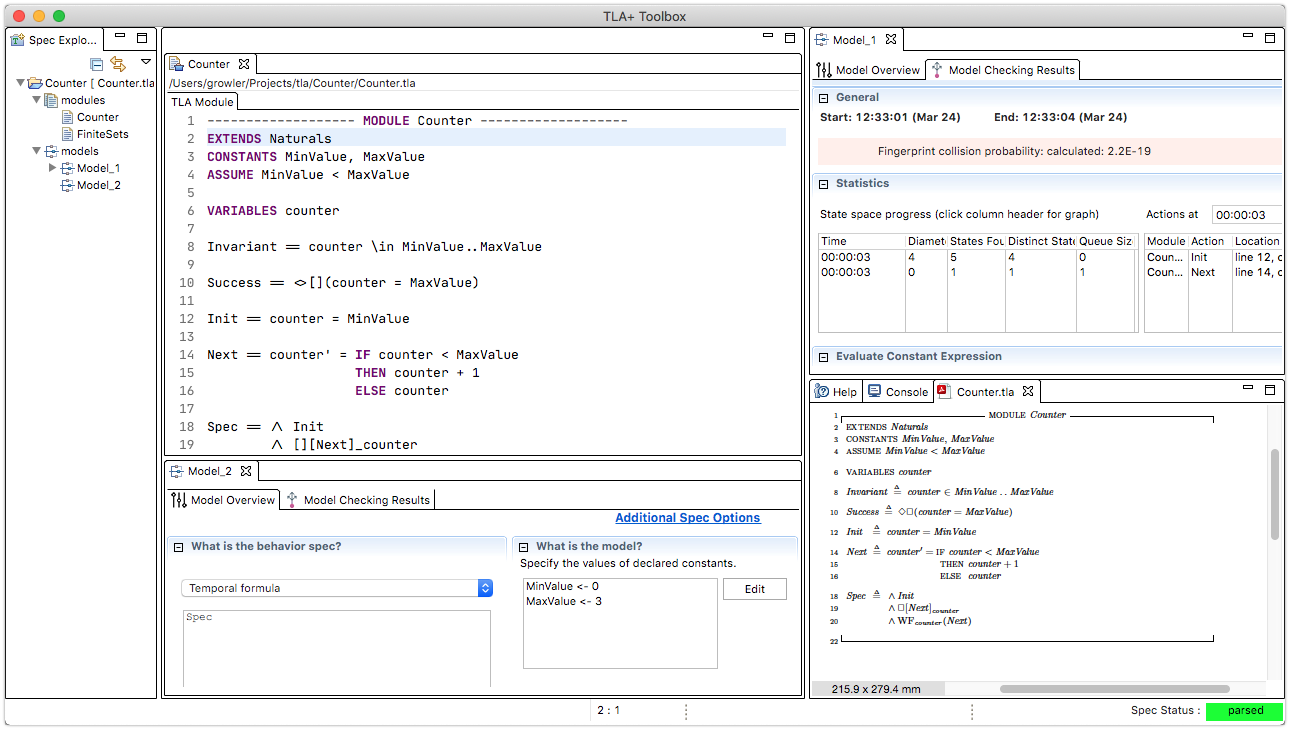
\includegraphics[keepaspectratio]{tla-toolbox-screenshot.png}};
    \draw[visible on=<2>,red] (1.49,2.50) rectangle (7.47,6.3);
    \draw[visible on=<3>,red] (1.49,0.28) rectangle (7.47,2.5);
    \draw[visible on=<4>,red] (7.49,3.30) rectangle (11.9,6.5);
  \end{tikzpicture}}%
\end{frame}

% Visual Studio Code
\begin{frame}[c]
  \centering\Large%
  \href{https://code.visualstudio.com/download}{VS Code}~/~%
  \href{https://marketplace.visualstudio.com/items?itemName=alygin.vscode-tlaplus}{TLA+ Support by Андрей Лыгин}%
  ~{\href{https://github.com/alygin}{@alygin}}\\%
  \resizebox{\textwidth}{!}{\begin{tikzpicture}[every node/.style={inner sep=0,outer sep=0}]
    \node at (0,0) [anchor=south west]{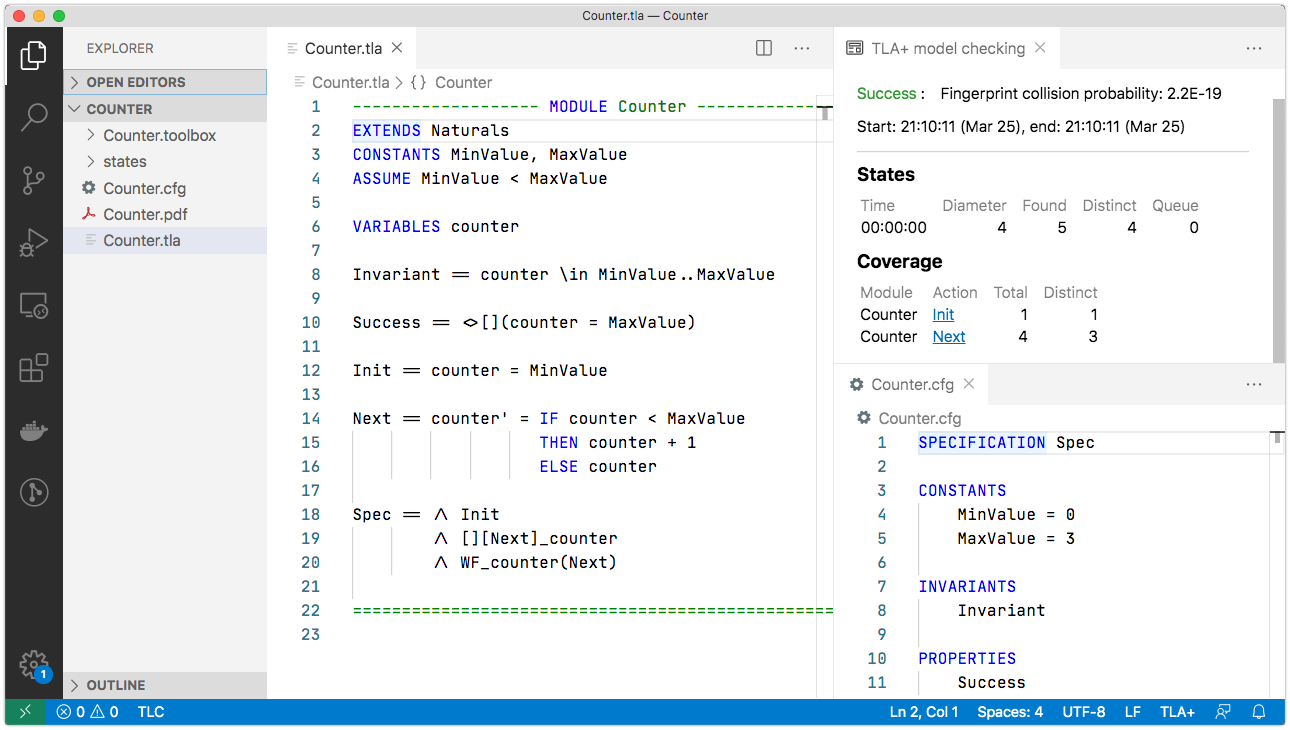
\includegraphics[keepaspectratio]{tla-vscode-screenshot.png}};
    \draw[visible on=<2>,red] (2.46,0.3)  rectangle (7.75,6.5);
    \draw[visible on=<3>,red] (7.75,0.3)  rectangle (11.93,3.38);
    \draw[visible on=<4>,red] (7.75,3.39) rectangle (11.93,6.5);
  \end{tikzpicture}}%
\end{frame}

% Демо -- счетчик
\begin{frame}[c]
  \centering
  {\Large\bf ДЕМО}\\[2ex]
  {\normalsize\ttfamily\textcolor{black!80}{00\_Counter.tla}}
\end{frame}

% PlusCal
\begin{frame}[t,fragile]
  \vspace{1ex}\centering{\Large\bf PlusCal}\\%
  \strut\only<1>{~}%
  \only<2>{Алгоритм}%
  \only<3>{Переменные}%
  \only<4>{Определения TLA+}%
  \only<5>{Процессы}%
  \only<6>{Метки}%
  \\%
  \only<2>{\setminted{highlightlines={4,26}}}%
  \only<3>{\setminted{highlightlines={6-8}}}%
  \only<4>{\setminted{highlightlines={10-12}}}%
  \only<5>{\setminted{highlightlines={14-18,20-24}}}%
  \only<6>{\setminted{highlightlines={15,21}}}%
  \begin{minipage}{\textwidth}
    \begin{columns}[T]
      \begin{column}{.45\textwidth}
        \inputcode[fontsize=\small,firstline=4,lastline=12]{tla}{01_PCDemo.tla}
      \end{column}
      \begin{column}{.45\textwidth}
        \inputcode[fontsize=\small,firstline=14,lastline=26]{tla}{01_PCDemo.tla}
      \end{column}
    \end{columns}
  \end{minipage}
\end{frame}

% PlusCal
\begin{frame}[t,fragile]
  \vspace{1ex}\centering{\Large\bf PlusCal}\\
  \strut{}Трансляция\\%
  \only<2>{\setminted{highlightlines={28,34}}}%
  \only<3>{\setminted{highlightlines={36}}}%
  \only<4>{\setminted{highlightlines={41,42}}}%
  \begin{minipage}{\textwidth}%
    \inputcode[fontsize=\small,firstline=27,lastline=31]{tla}{01_PCDemo.tla}%
    \vspace{-1.5ex}%
    \inputcode[fontsize=\small,firstline=34,lastline=42]{tla}{01_PCDemo.tla}%
  \end{minipage}
\end{frame}

\begin{frame}[t,fragile]
  \vspace{1ex}\centering{\Large\bf PlusCal}\\
  \strut{}Трансляция\\%
  \only<2>{\setminted{highlightlines={44,51}}}%
  \only<3>{\setminted{highlightlines={47,54}}}%
  \begin{minipage}{\textwidth}%
    \inputcode[fontsize=\small,firstline=44,lastline=56]{tla}{01_PCDemo.tla}%
  \end{minipage}
\end{frame}

\begin{frame}[t,fragile]
  \vspace{1ex}\centering{\Large\bf PlusCal}\\
  \strut{}Трансляция\\%
  \only<2>{\setminted{highlightlines={59,60,69}}}%
  \begin{minipage}{\textwidth}%
    \inputcode[fontsize=\small,firstline=58,lastline=69]{tla}{01_PCDemo.tla}%
  \end{minipage}
\end{frame}

% Демо -- два агента
\begin{frame}[c]
  \centering{\Large\bf ДЕМО}\\[2ex]%
  {\normalsize\ttfamily\textcolor{black!80}{01\_PCDemo.tla}}
\end{frame}

% TLA+ Toolbox CLI
\definecolor{shellbgcolor}{rgb}{1,0.99,0.96}
\begin{frame}[c,fragile]
  {\centering\Large TLA+ Toolbox CLI\\}
  \begin{tcolorbox}[colback=shellbgcolor,boxrule=.25pt]%
    \scriptsize%
    \begin{Verbatim}[commandchars=\\\{\}]
\textcolor[HTML]{D78600}{growler@macbook}:\textcolor{green!90!black}{$} tlc -dump dot,colorized 01_PCDemo.dot 01_PCDemo.tla
\textcolor{black!50}{Computing initial states...}
\textcolor{black!50}{Finished computing initial states: 1 distinct state generated.}
\textcolor{black!50}{Checking 2 branches of temporal properties for the complete state space}
\textcolor{black!50}{  with 10 total distinct states}
\textcolor{black!50}{Finished checking temporal properties}
\textcolor{black!50}{Model checking completed. No error has been found.}
\textcolor{black!50}{  Estimates of the probability that TLC did not check all reachable states}
\textcolor{black!50}{  because two distinct states had the same fingerprint:}
\textcolor{black!50}{  calculated (optimistic):  val = 5.4E-19}
\textcolor{black!50}{7 states generated, 5 distinct states found, 0 states left on queue.}
\textcolor[HTML]{D78600}{growler@macbook}:\textcolor{green!90!black}{$} dot -Tsvg 01_PCDemo.dot -o 01_PCDemo.svg
\textcolor[HTML]{D78600}{growler@macbook}:\textcolor{green!90!black}{$}
    \end{Verbatim}
  \end{tcolorbox}
\end{frame}

% TLA+ ToolBox -- States diagram
\begin{frame}[c]
  \begin{center}
    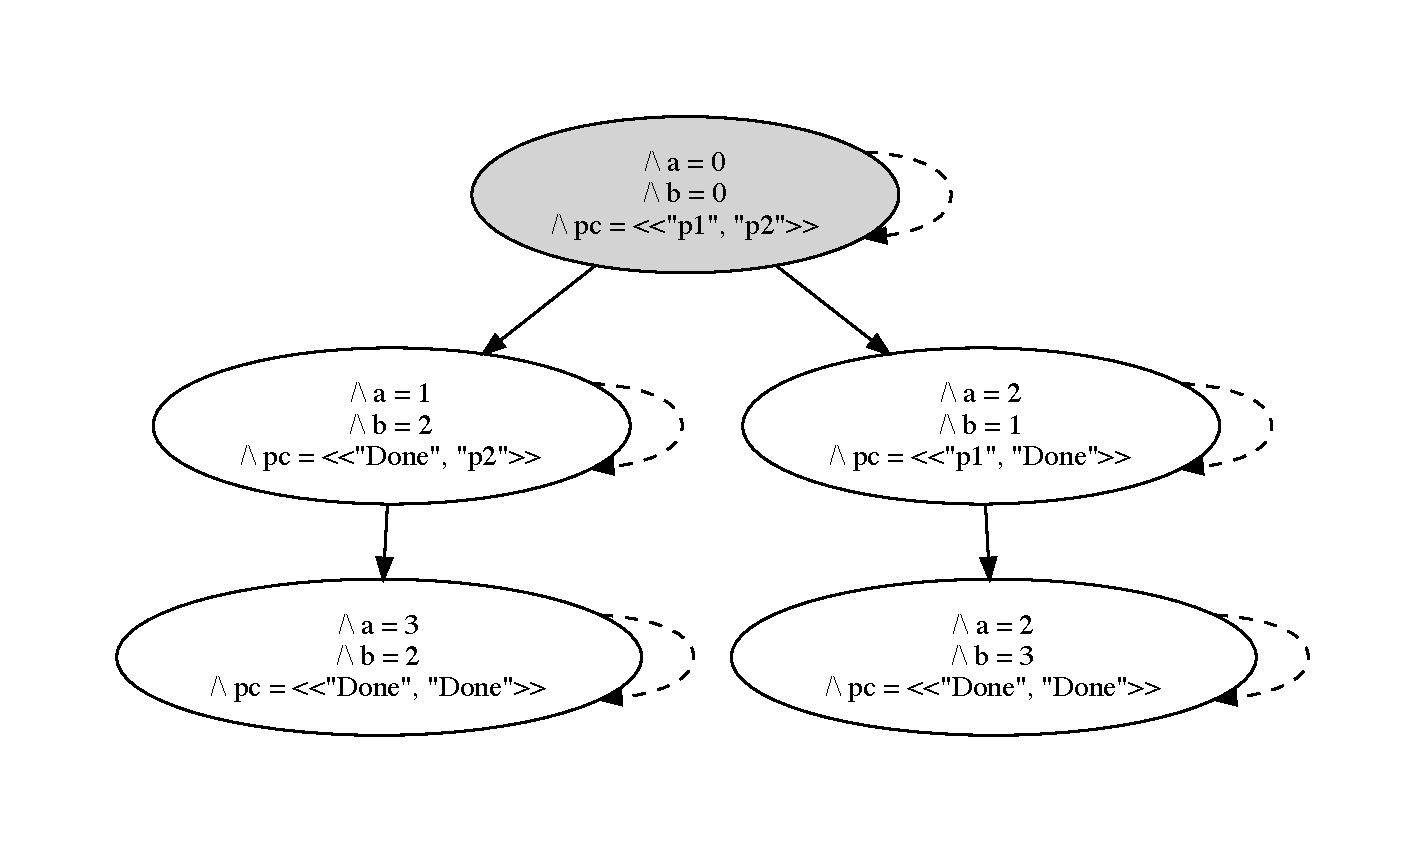
\includegraphics[keepaspectratio, height=.9\textheight]{01_PCDemo.pdf}%
  \end{center}
\end{frame}

% PlusCal -- атомарность
\begin{frame}[c,fragile]
  \begin{overlayarea}{\textwidth}{7ex}
    \begin{minipage}{\textwidth}
      \centering%
      {\Large\bf PlusCal\\}%
      {Атомарность}%
    \end{minipage}%
  \end{overlayarea}%
  \setminted{highlightlines={18,19,24,25}}%
  \begin{minipage}{\textwidth}
    \begin{columns}[T]
      \begin{column}{.45\textwidth}
        \inputcode[fontsize=\small,firstline=4,lastline=14]{tla}{02_PCDemo.tla}
      \end{column}
      \begin{column}{.45\textwidth}
        \inputcode[fontsize=\small,firstline=16,lastline=28]{tla}{02_PCDemo.tla}
      \end{column}
    \end{columns}
  \end{minipage}
\end{frame}

% Демо -- гонки
\begin{frame}[c]
  \centering
  {\Large\bf ДЕМО}\\[2ex]
  {\normalsize\ttfamily\textcolor{black!80}{02\_PCDemo.tla}}
\end{frame}

\newcommand{\vhl}[2]{\alt<#1>{\bf\ttfamily\textcolor{red!90!black}{#2}}{#2}}
% Демо -- гонки
\begin{frame}[c,fragile]
  \begin{tcolorbox}[colback=shellbgcolor,boxrule=.25pt]%
  \centering\tiny%
  \begin{Verbatim}[commandchars=!\{\}]
    !vhl{2-}{Error: Temporal properties were violated.}

    !vhl{3-}{Error: The following behavior constitutes a counter-example:}
    
    State 1: <Initial predicate>
    /\ a = 0
    /\ b = 0
    /\ pc = <<"p1_1", "p2_1">>
    
    State 2: <p1_1 line 48, col 9 to line 51, col 17 of module 02_PCDemo>
    /\ a = 1
    /\ b = 0
    /\ pc = <<"p1_2", "p2_1">>
    
    State 3: <p2_1 line 60, col 9 to line 63, col 17 of module 02_PCDemo>
    /\ a = 1
    /\ b = 2
    /\ pc = <<"p1_2", "p2_2">>
    
    State 4: <p2_2 line 65, col 9 to line 68, col 17 of module 02_PCDemo>
    /\ a = 3
    /\ b = 2
    /\ pc = <<"p1_2", "Done">>
    
    !vhl{4}{State 5: <p1_2 line 53, col 9 to line 56, col 17 of module 02_PCDemo>}
    !vhl{4}{/\ a = 3}
    !vhl{4}{/\ b = 4}
    /\ pc = <<"Done", "Done">>
  \end{Verbatim}
\end{tcolorbox}
\end{frame}

% Демо -- гонки
\begin{frame}[c]
  \centering\resizebox{\textwidth}{!}{%
  \begin{tikzpicture}
    \node[anchor=south west,inner sep=0] at (0,0) {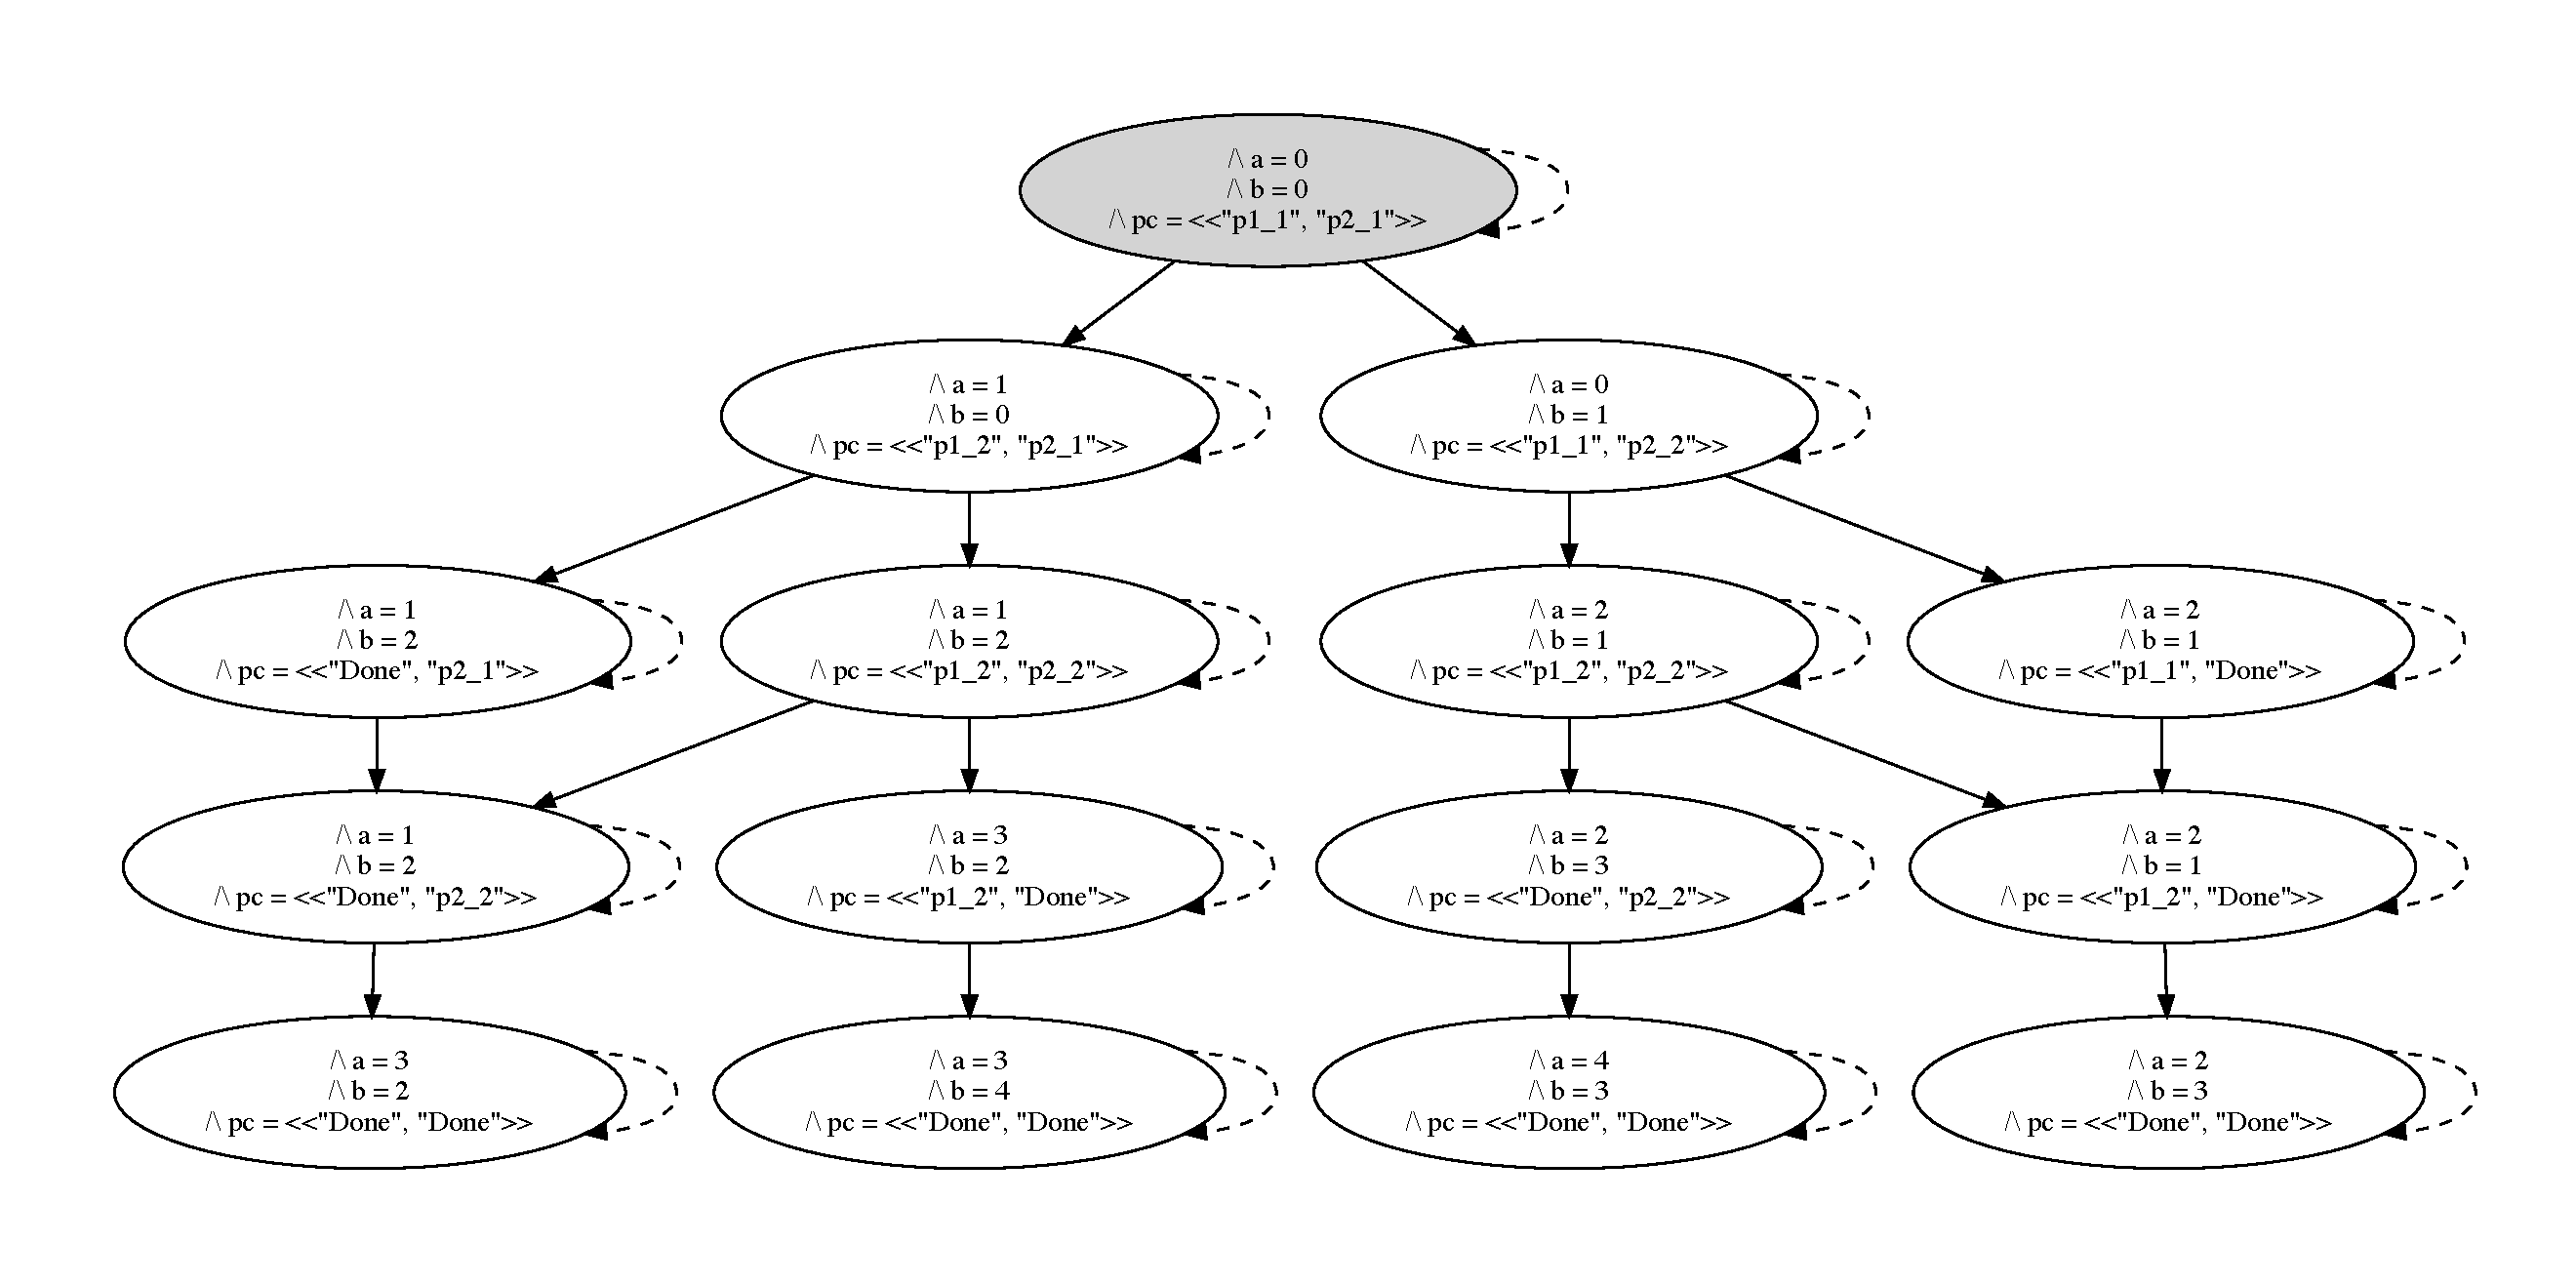
\includegraphics{02_PCDemo.pdf}};
    \draw[visible on=<2>,ultra thick,red,rounded corners] (12.2,1.5) rectangle (32.7,5.25);
  \end{tikzpicture}}%
\end{frame}

\begingroup
\renewcommand*{\arraystretch}{1.3}
\def\scmd#1{\textbackslash\relax#1}%
% Множества
\begin{frame}[t,fragile]
  \vspace{2ex}%
  \centering{\Large\bf Sets (Множества)\\}\strut\\%
  \begin{center}\begin{minipage}{.6\textwidth}
  \begin{tabular}{>{\begingroup\ttfamily\normalsize}l<{\endgroup}}
    Procs == \{1, 5, 8\}                       \\
    Ops == \{"inc", "dec"\}                    \\
    Vals == 1..MaxValue                        \\\pause
    Cmd == Ops \scmd{union} \{NULL\}           \\
    \{1, 2\} \scmd{intersect} \{2, 3\} = \{2\} \\
    Var \scmd{in} 1..10                        \\
    ASSUME Var \scmd{notin} Procs              \\\pause
    TRUE \scmd{in} BOOLEAN                     \\
    "string" \scmd{in} STRING                  \\
    UNION \{\{1, 2\}, \{2, 3\}\} = \{1, 2, 3\}
  \end{tabular}
  \end{minipage}\end{center}
\end{frame}

\begin{frame}[t,fragile]
  \vspace{2ex}%
  \centering{\Large\bf Tuples (Кортежи)\\}\strut\\%
  \begin{center}\begin{minipage}{.6\textwidth}
  \begin{tabular}{>{\begingroup\ttfamily\normalsize}l<{\endgroup}}
    a == <<1, 5, 8>>                           \\
    a[2] = 5                                   \\\pause
    Len(a) = 3                                 \\
    Head(a) = 1                                \\
    Tail(a) = <<5, 8>>                         \\
    SubSeq(a, 1, 2) = <<1, 5>>                 \\\pause
    <<1, 2>> \scmd{o} <<4, 8>> = <<1, 2, 4, 8>>\\
    a := Append(a, 5)                          \\
    a[i] := i                                  \\
  \end{tabular}    
  \end{minipage}\end{center}
\end{frame}

\begin{frame}[t,fragile]
  \vspace{2ex}%
  \centering{\Large\bf Records (Записи)\\}\strut\\%
  \begin{center}\begin{minipage}{.6\textwidth}
  \begin{tabular}{>{\begingroup\ttfamily\normalsize}l<{\endgroup}}
    s == [rdy|->0, ack|->0, val|->0]       \\
    s.rdy = 0                              \\
    s["ack"] = 0                           \\\pause
    "a" :> 1 = [a|->1]                     \\\relax
    [a|->1] @@ [b|->2] = [a|->1, b|->2]    \\\pause
    s.ack := 1                             \\
    p.a := p.b || p.b = p.a                \\
  \end{tabular}  
  \end{minipage}\end{center}  
\end{frame}

\begin{frame}[t,fragile]
  \vspace{2ex}%
  \centering{\Large\bf Functions (Функции)\\}\strut\\%
  \begin{center}\begin{minipage}{.6\textwidth}
  \begin{tabular}{>{\begingroup\ttfamily\normalsize}l<{\endgroup}}
    Squares == [n \scmd{in} 1..Nat |-> n * n] \\
    Squares[2] = 4                         \\
    DOMAIN Squares = 1..Nat                \\\pause
    s == [rdy|->0, ack|->0, val|->0]       \\
    DOMAIN s = \{"ack", "rdy", "val"\}     \\\pause
    DOMAIN <<5, 6, 7>> = 1..3              
  \end{tabular}
  \end{minipage}\end{center}
\end{frame}
\endgroup

% PlusCal Go Channel
\begin{frame}[t,fragile]
  \centering{\Large\bf Go Channel\\}~\\[1ex]%
  \inputcode[fontsize=\scriptsize,firstline=9,lastline=22]{go}{03_gochannel_test.go}
\end{frame}

% PlusCal Go Channel
\begin{frame}[t,fragile]
  \centering{\Large\bf Go Channel\\}~\\[1ex]%
  \only<2>{\setminted{highlightlines={7}}}%
  \only<3>{\setminted{highlightlines={10}}}%
  \only<4>{\setminted{highlightlines={12}}}%
  \inputcode[fontsize=\scriptsize,firstline=1,lastline=13]{tla}{03_GoChannel.tla}
\end{frame}

% PlusCal Go Channel -- cont.
\begin{frame}[t,fragile]
  \centering{\Large\bf Go Channel\\}~\\[1ex]%
  \only<2>{\setminted{highlightlines={18,25}}}%
  \only<3>{\setminted{highlightlines={19,22,33,36}}}%
  \only<4>{\setminted{highlightlines={31,39}}}%
  \only<5>{\setminted{highlightlines={32,35,38}}}%
  \only<6>{\setminted{highlightlines={20,23,34}}}%
  \only<7>{\setminted{highlightlines={17-20}}}%
  \only<8>{\setminted{highlightlines={21-23}}}%
  \only<9>{\setminted{highlightlines={24-26}}}%
  \only<10>{\setminted{highlightlines={32-34}}}%
  \only<11>{\setminted{highlightlines={35-38}}}%
  \begin{columns}[T,onlytextwidth]%
    \begin{column}{.5\textwidth}%
      \inputcode[fontsize=\scriptsize,firstline=15,lastline=27]{tla}{03_GoChannel.tla}
    \end{column}%
    \begin{column}{.5\textwidth}%
      \inputcode[fontsize=\scriptsize,firstline=29,lastline=42]{tla}{03_GoChannel.tla}
    \end{column}%
  \end{columns}
\end{frame}

% Демо -- Go Channel
\begin{frame}[c]
  \centering
  {\Large\bf ДЕМО}\\[2ex]
  {\normalsize\ttfamily\textcolor{black!80}{03\_GoChannel.tla}}
\end{frame}

% PlusCal -- Макросы
\begin{frame}[t,fragile]
  \begin{minipage}{\textwidth}
      \centering%
      {\Large\bf PlusCal\\}%
      Макросы%
  \end{minipage}\\[1ex]%
  \only<2>{\setminted{highlightlines={14-19,21-25}}}%
  \only<3>{\setminted{highlightlines={27-34}}}%
  \only<4>{\setminted{highlightlines={36-40}}}%
  \begin{minipage}{\textwidth}
    \begin{columns}[T]
      \begin{column}{.5\textwidth}
        \inputcode[fontsize=\scriptsize,firstline=14,lastline=25]{tla}{04_GoChannel.tla}
      \end{column}
      \begin{column}{.5\textwidth}
        \inputcode[fontsize=\scriptsize,firstline=27,lastline=40]{tla}{04_GoChannel.tla}
      \end{column}
    \end{columns}
  \end{minipage}
\end{frame}

% Go Channel w/ macros
\begin{frame}[t,fragile]
  \begin{minipage}{\textwidth}
      \centering%
      {\Large\bf Go Channel\\}~%
  \end{minipage}\\[2ex]%
  \only<2>{\setminted{highlightlines={7}}}%
  \only<3>{\setminted{highlightlines={46,59}}}%
  \only<4>{\setminted{highlightlines={11}}}%
  \only<5>{\setminted{highlightlines={47,48,50}}}%
  \only<6>{\setminted{highlightlines={57}}}%
  \begin{minipage}{\textwidth}
    \begin{columns}[T]
      \begin{column}{.5\textwidth}
        \inputcode[fontsize=\scriptsize,firstline=7,lastline=7]{tla}{04_GoChannel.tla}%
        \vspace{-1ex}%
        \inputcode[fontsize=\scriptsize,firstline=11,lastline=11]{tla}{04_GoChannel.tla}%
        \vspace{-1ex}%
        \inputcode[fontsize=\scriptsize,firstline=42,lastline=51]{tla}{04_GoChannel.tla}%
      \end{column}
      \begin{column}{.5\textwidth}
        \inputcode[fontsize=\scriptsize,firstline=53,lastline=64]{tla}{04_GoChannel.tla}%
      \end{column}
    \end{columns}
  \end{minipage}
\end{frame}

% Демо -- Go Channel w/macros
\begin{frame}[c]
  \centering
  {\Large\bf ДЕМО}\\[2ex]
  {\normalsize\ttfamily\textcolor{black!80}{04\_GoChannel.tla}}
\end{frame}

% Go Channel Bug
\begin{frame}[t,fragile]
  \begin{minipage}{\textwidth}
      \centering%
      {\Large\bf Go Channel Bug\\}~%
  \end{minipage}\\[2ex]%
  \begin{minipage}{\textwidth}
    \begin{columns}[T]
      \begin{column}{.5\textwidth}
        \only<3>{\setminted{highlightlines={19,20}}}%
        {\scriptsize\textcolor{black!50}{\Verb|05_channelbug_test.go|}}\\[-1ex]
        \inputcode[tabsize=2,fontsize=\scriptsize,firstline=10,lastline=22]{go}{05_channelbug_test.go}%
      \end{column}
      \begin{column}{.5\textwidth}<2->
        \only<3>{\setminted{highlightlines={35,36}}}%
        {\scriptsize\textcolor{black!50}{\Verb|05_ChannelBug.tla|}}\\[-1ex]
        \inputcode[fontsize=\scriptsize,firstline=24,lastline=38]{tla}{05_ChannelBug.tla}%
      \end{column}
    \end{columns}
  \end{minipage}
\end{frame}

% Демо -- Go Channel Bug
\begin{frame}[c]
  \centering
  {\Large\bf ДЕМО}\\[2ex]
  {\normalsize\ttfamily\textcolor{black!80}{05\_ChannelBug.tla}}
\end{frame}

% Демо -- гонки
\begin{frame}[c,fragile]
  \begin{tcolorbox}[colback=shellbgcolor,boxrule=.25pt]%
  \centering\tiny%
  \begin{Verbatim}[commandchars=!\{\}]
!vhl{2-}{Error: Deadlock reached.}
!vhl{3-}{Error: The behavior up to this point is:}
State 1: <Initial predicate>
/\ ch = [open |-> TRUE, val |-> NULL, sent |-> FALSE, rcvd |-> FALSE]
/\ pc = [processor |-> "Proc_1", receiver |-> "Rec_1"]
/\ rslt = NULL

State 2: <Proc_1 line 55, col 11 to line 59, col 25 of module 05_ChannelBug>
/\ ch = [open |-> TRUE, val |-> "result", sent |-> TRUE, rcvd |-> FALSE]
/\ pc = [processor |-> "Proc_2", receiver |-> "Rec_1"]
/\ rslt = NULL

State 3: <Rec_1 line 69, col 10 to line 78, col 52 of module 05_ChannelBug>
/\ ch = [open |-> TRUE, val |-> "result", sent |-> TRUE, rcvd |-> FALSE]
!vhl{3-}{/\ pc = [processor |-> "Proc_2", receiver |-> "Done"]}
/\ rslt = NULL

7 states generated, 6 distinct states found, 1 states left on queue.
  \end{Verbatim}
\end{tcolorbox}
\end{frame}

% Unbound Queue Bugged (go)
\begin{frame}[t,fragile]
  \begin{minipage}{\textwidth}
      \centering%
      {\Large\bf Go Unbound Queue\\}~%
  \end{minipage}\\[2ex]%
  \begin{minipage}{\textwidth}
    \begin{columns}[T]
      \begin{column}{.5\textwidth}
        \inputcode[tabsize=2,fontsize=\scriptsize,firstline=8,lastline=23]{go}{06_unboundqueue_test.go}%
      \end{column}
      \begin{column}{.5\textwidth}
        \inputcode[tabsize=2,fontsize=\scriptsize,firstline=24,lastline=32]{go}{06_unboundqueue_test.go}%
        \vspace{-1ex}%
        \inputcode[tabsize=2,fontsize=\scriptsize,firstline=60,lastline=62]{go}{06_unboundqueue_test.go}%
      \end{column}
    \end{columns}
  \end{minipage}
\end{frame}

% Unbound Queue Bugged (TLA)
\begin{frame}[t,fragile]
  \begin{minipage}{\textwidth}
      \centering%
      {\Large\bf Go Unbound Queue\\}~%
  \end{minipage}\\[2ex]%
  \begin{minipage}{\textwidth}
    \begin{columns}[T]
      \begin{column}{.5\textwidth}
        \inputcode[tabsize=2,fontsize=\scriptsize,firstline=56,lastline=68]{tla}{06_UnboundQueue.tla}%
      \end{column}
      \begin{column}{.5\textwidth}
        \inputcode[tabsize=2,fontsize=\scriptsize,firstline=69,lastline=78]{tla}{06_UnboundQueue.tla}%
      \end{column}
    \end{columns}
  \end{minipage}
\end{frame}

% Демо -- Unbound Queue Bugged
\begin{frame}[c]
  \centering
  {\Large\bf ДЕМО}\\[2ex]
  {\normalsize\ttfamily\textcolor{black!80}{06\_UnboundQueue.tla}}
\end{frame}

% Демо -- Unbound Queue Bugged
\begin{frame}[c,fragile]
  \begin{tcolorbox}[colback=shellbgcolor,boxrule=.25pt]%
  \centering\tiny%
  \begin{Verbatim}[commandchars=!\{\}]
    !vhl{2-}{Error: Temporal properties were violated.}
    !vhl{2-}{Error: The following behavior constitutes a counter-example:}
    ...
    State 30: <Consume line 138, col 12 to line 146, col 66 of module 06_UnboundQueue>
    /\ buffer = <<3>>
    /\ i = 3
    /\ j = NULL
    /\ k = NULL
    /\ pc = [buffer |-> "Done", producer |-> "Done", consumer |-> "Consumer_1"]
    /\ recvd = <<1, 2>>
    /\ inpCh = [sent |-> FALSE, open |-> FALSE, val |-> NULL, rcvd |-> FALSE]
    /\ outCh = [sent |-> FALSE, open |-> FALSE, val |-> NULL, rcvd |-> FALSE]
    /\ sent = <<1, 2, 3>>
    /\ id = 4
    
    State 31: <Consumer_1 line 148, col 15 to line 154, col 72 of module 06_UnboundQueue>
    !vhl{3-}{/\ buffer = <<3>>}
    /\ i = 3
    /\ j = NULL
    /\ k = NULL
    /\ pc = [buffer |-> "Done", producer |-> "Done", consumer |-> "Done"]
    !vhl{3-}{/\ recvd = <<1, 2>>}
    /\ inpCh = [sent |-> FALSE, open |-> FALSE, val |-> NULL, rcvd |-> FALSE]
    /\ outCh = [sent |-> FALSE, open |-> FALSE, val |-> NULL, rcvd |-> FALSE]
    !vhl{3-}{/\ sent = <<1, 2, 3>>}
    /\ id = 4
    
    State 32: Stuttering
    !vhl{4-}{406 states generated, 213 distinct states found, 0 states left on queue.}
  \end{Verbatim}
\end{tcolorbox}
\end{frame}

% Unbound Queue Fixed (TLA)
\begin{frame}[t,fragile]
  \begin{minipage}{\textwidth}
      \centering%
      {\Large\bf Go Unbound Queue (fixed)\\}~%
  \end{minipage}\\[1ex]%
  \begin{minipage}{\textwidth}
    \begin{columns}[T]
      \begin{column}{.5\textwidth}
        \inputcode[tabsize=2,fontsize=\scriptsize,firstline=54,lastline=67,%
            highlightlines={56,66}%
        ]{tla}{07_UnboundQueue.tla}%
      \end{column}
      \begin{column}{.5\textwidth}
        \inputcode[tabsize=2,fontsize=\scriptsize,firstline=68,lastline=81,%
          highlightlines={75-78}%
        ]{tla}{07_UnboundQueue.tla}%
      \end{column}
    \end{columns}
  \end{minipage}
\end{frame}

% Демо -- Unbound Queue Fixed
\begin{frame}[c]
  \centering
  {\Large\bf ДЕМО}\\[2ex]
  {\normalsize\ttfamily\textcolor{black!80}{07\_UnboundQueue.tla}}
\end{frame}

% Unbound Queue Fixed (go)
\begin{frame}[t,fragile]
  \begin{minipage}{\textwidth}
      \centering%
      {\Large\bf Go Unbound Queue (fixed)\\}~%
  \end{minipage}\\[1ex]%
  \begin{minipage}{\textwidth}
    \begin{columns}[T]
      \begin{column}{.5\textwidth}
        \inputcode[tabsize=2,fontsize=\scriptsize,firstline=5,lastline=20,%
          highlightlines={7,16-20}%
        ]{go}{07_unboundqueue_test.go}%
      \end{column}
      \begin{column}{.5\textwidth}
        \inputcode[tabsize=2,fontsize=\scriptsize,firstline=21,lastline=37,%
          highlightlines={30-33}%
        ]{go}{07_unboundqueue_test.go}%
      \end{column}
    \end{columns}
  \end{minipage}
\end{frame}

\begin{frame}
  \centering\Large\bf{А на практике?}
\end{frame}

\begin{frame}[c]
  \centering\large%
  \vfill%
  \begin{beamercolorbox}{}
    Amazon Web Services \href{http://lamport.azurewebsites.net/tla/formal-methods-amazon.pdf}{%
    \textcolor{blue}{успешно использует TLA+}}\textsuperscript{1} с 2011 года\\[2ex]%
    \hfill\begin{minipage}{.95\textwidth}
      \normalsize\itshape%
      ``At AWS, formal methods have been a big success. They have helped us prevent subtle, serious bugs
      from reaching production, bugs that we would not have found via any other technique.''
    \end{minipage}
    \strut\\[2ex]
    \onslide<2>{
    Microsoft использует TLA+%
    \href{https://www.microsoft.com/en-us/research/search/?q=TLA\%2B}%
    {\textcolor{blue}{во многих проектах}}\textsuperscript{2},
    включая Azure
    \href{https://docs.microsoft.com/en-us/azure/cosmos-db/consistency-levels}%
    {\textcolor{blue}{CosmosDB}}\textsuperscript{3}%
    \\[2ex]%
    \hfill\begin{minipage}{.95\textwidth}
      \normalsize\itshape%
      ``TLA+ is not yet a prerequisite for our hiring. 
      However, a candidate's knowledge of TLA+ is given significant weight in
      our evaluation.  To us, it is a great indicator of those who really care
      about quality and correctness.''
    \end{minipage}%
    }
  \end{beamercolorbox}
  \vspace{5ex}%  
  \begin{minipage}{\textwidth}
    \scriptsize\color{black!60}%
    \onslide<1->{%
      1. \href{http://lamport.azurewebsites.net/tla/formal-methods-amazon.pdf}{%
        http://lamport.azurewebsites.net/tla/formal-methods-amazon.pdf}\\
    }%
    \onslide<2->{%
      2. \href{https://www.microsoft.com/en-us/research/search/?q=TLA\%2B}{%
        https://www.microsoft.com/en-us/research/search/?q=TLA\%2B}\\
      3. \href{https://docs.microsoft.com/en-us/azure/cosmos-db/consistency-levels}{%
        https://docs.microsoft.com/en-us/azure/cosmos-db/consistency-levels}\\
    }%
  \end{minipage}
\end{frame}

\begin{frame}[c]
  \centering\large%
  \vfill%
  \begin{beamercolorbox}{}
    MongoDB для
    \href{https://conf.tlapl.us/07_-_TLAConf19_-_William_Schultz_-_Fixing_a_MongoDB_Replication_Protocol_Bug_with_TLA.pdf}{%
      \textcolor{blue}{поиска}}\textsuperscript{1} ошибок в
    \href{https://github.com/will62794/mongo-repl-tla-models}{%
      \textcolor{blue}{протоколе}}\textsuperscript{2}
    репликации
    \\[2ex]%
    \hfill\begin{minipage}{.95\textwidth}
      \normalsize\itshape%
      ``We expect that formally modeling our system upfront could have saved
      100s of hours of engineering time.''
    \end{minipage}
    \strut\\[2ex]
    \onslide<2>{
    CockroachDB для
    \href{https://www.cockroachlabs.com/blog/parallel-commits/}%
    {\textcolor{blue}{спецификации}}\textsuperscript{3} протокола
    \href{https://github.com/cockroachdb/cockroach/tree/master/docs/tla-plus}%
    {\textcolor{blue}{распределенных транзакций}}\textsuperscript{4}%
    \\[2ex]%
    \hfill\begin{minipage}{.95\textwidth}
      \normalsize\itshape%
      ``We found that the process of writing this specification 
      gave us more confidence in the Parallel Commit protocol itself
      and in its integration into CockroachDB.''
    \end{minipage}    
    }%
  \end{beamercolorbox}
  \vspace{5ex}%  
  \begin{minipage}{\textwidth}
    \scriptsize\color{black!60}%
    \onslide<1->{%
      1. \href{https://conf.tlapl.us/07_-_TLAConf19_-_William_Schultz_-_Fixing_a_MongoDB_Replication_Protocol_Bug_with_TLA.pdf}{%
        conf.tlapl.us/07\_-\_TLAConf19\_-\_William\_Schultz\_-\_Fixing\_a\_MongoDB\_Replication\_Protocol\_Bug\_with\_TLA.pdf}\\
      2. \href{https://github.com/will62794/mongo-repl-tla-models}{%
        github.com/will62794/mongo-repl-tla-models}\\
    }%
    \onslide<2->{%
      3. \href{https://www.cockroachlabs.com/blog/parallel-commits/}{%
        www.cockroachlabs.com/blog/parallel-commits}\\
      4. \href{https://github.com/cockroachdb/cockroach/tree/master/docs/tla-plus}{%
        github.com/cockroachdb/cockroach/tree/master/docs/tla-plus}\\
    }%
  \end{minipage}
\end{frame}

\begin{frame}
  \centering\Large\bf{С чего начать?}
\end{frame}

\begin{frame}[c]
  \begin{columns}
    \begin{column}{.45\textwidth}
      \centering
      \href{https://www.apress.com/gp/book/9781484238288}{%
        
\includegraphics[keepaspectratio, height=.85\textheight]{practical-tla-cover.pdf}
      }
    \end{column}
    \begin{column}{.45\textwidth}
      \href{https://www.apress.com/gp/book/9781484238288}{%
        {\Large\bf Practical TLA+}\\
        {\large\bf Planning Driven Development}\\
        {\normalsize by Hillel Wayne\\Apress, 2018}
      }\\
      \vspace{3ex}
      \large
      PlusCal, идеально для вхождения в тему!
    \end{column}
  \end{columns}
\end{frame}

\begin{frame}[c]
  \begin{columns}
    \begin{column}{.45\textwidth}
      \centering
      \href{https://lamport.azurewebsites.net/tla/book.html\#download}{%
        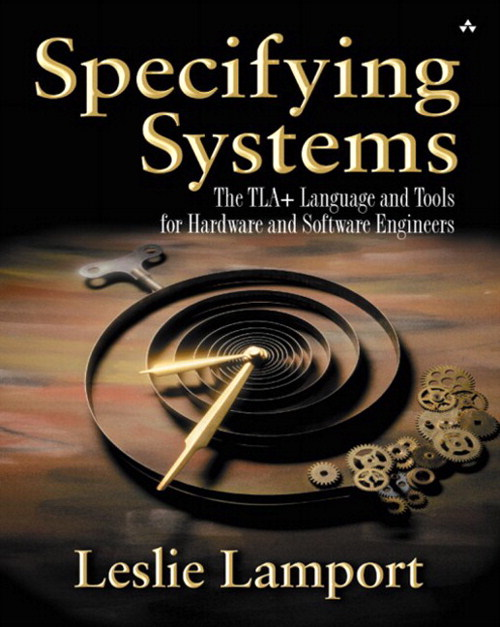
\includegraphics[keepaspectratio, height=.85\textheight]{specifying-systems-cover.jpg}
      }
    \end{column}
    \begin{column}{.45\textwidth}
      \href{https://lamport.azurewebsites.net/tla/book.html\#download}{%
        {\Large\bf Specifying Systems}\\
        {\large\bf The TLA+ Language and Tools for Hardware and Software Engineers}\\
        {\normalsize by Leslie Lamport\\Addison-Wesley Professional, 2002}
      }\\
      \vspace{3ex}
      \large
      TLA+, обязательно иметь под рукой\\
      \vspace{3ex}
      (последняя версия всегда доступна на сайте Лэмпорта, бесплатно!)
    \end{column}
  \end{columns}
\end{frame}

\begin{frame}[c]
  \begin{columns}
    \begin{column}{.45\textwidth}
      \centering
      \href{http://lamport.azurewebsites.net/video/videos.html}{%
        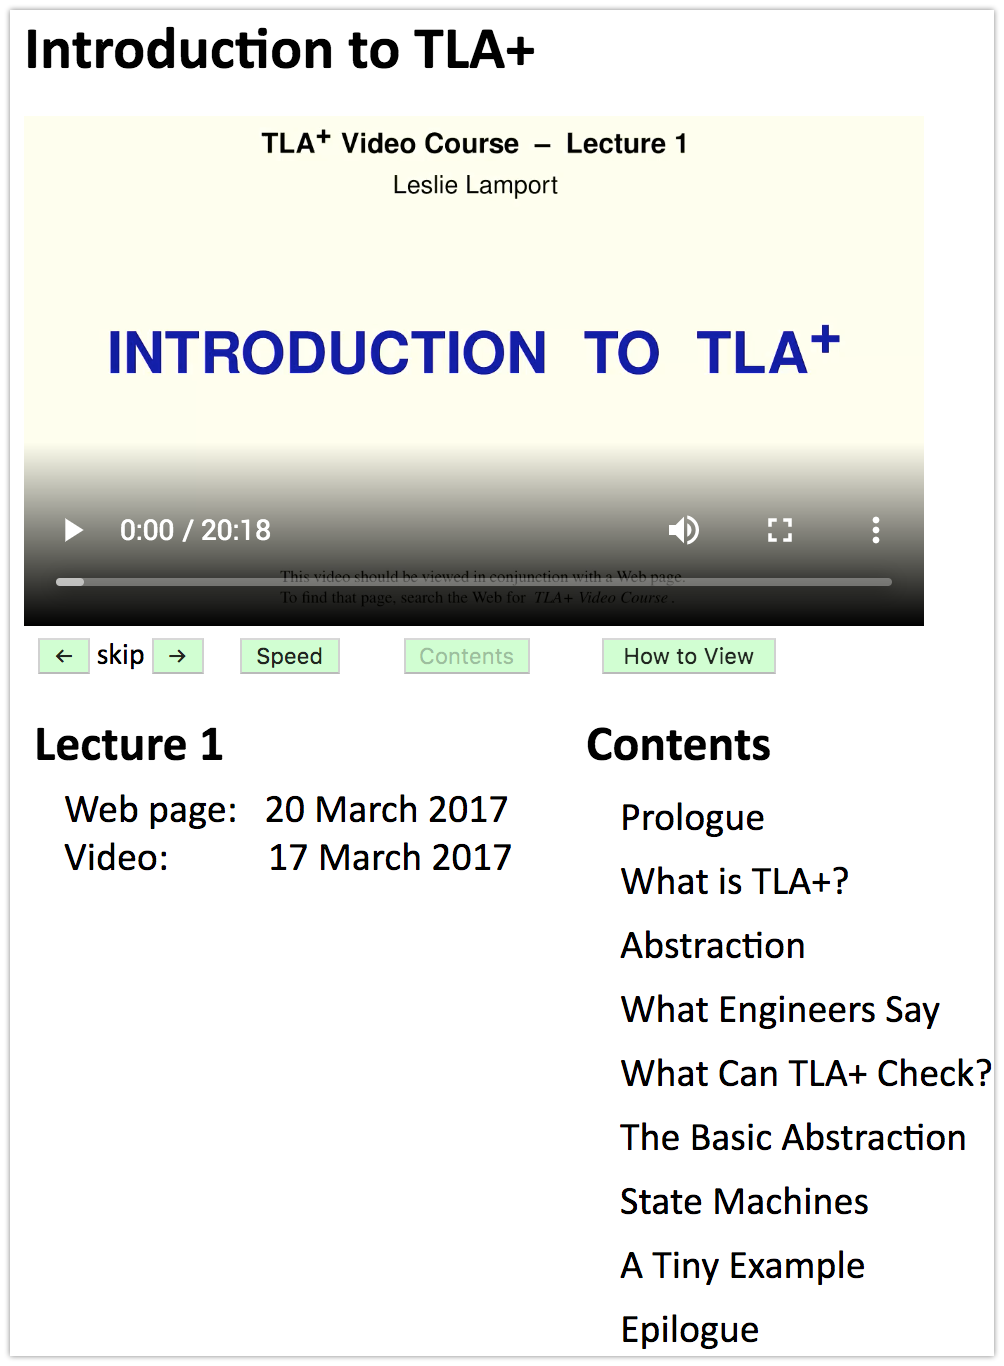
\includegraphics[keepaspectratio, height=.85\textheight]{tla-video-course-cover.png}
      }
    \end{column}
    \begin{column}{.45\textwidth}
      \href{http://lamport.azurewebsites.net/video/videos.html}{%
        {\Large\bf TLA+ Video Course}\\
        {\normalsize by Leslie Lamport}\\
        {\tiny \nolinkurl{lamport.azurewebsites.net/video/videos.html}}
      }\\
      \vspace{3ex}
      \large
      3.5 часа TLA+, обязательно посмотреть\\
      \vspace{3ex}
      (Лэмпорт прекрасный лектор!)
    \end{column}
  \end{columns}
\end{frame}

\begin{frame}[c]
  \centering\large%
  \vfill%
  \begin{beamercolorbox}{}
    Lamport TLA+ Site: \href{https://lamport.azurewebsites.net/tla/tla.html}{\textcolor{blue}{https://lamport.azurewebsites.net/tla/tla.html}}\\[2ex]
    Learn TLA+: \href{https://learntla.com/}{\textcolor{blue}{https://learntla.com}}\\[2ex]
    google group: \href{https://groups.google.com/forum/\#!forum/tlaplus}{\textcolor{blue}{https://groups.google.com/forum/\#!forum/tlaplus}}\\[2ex]
    reddit: \href{https://www.reddit.com/r/tlaplus/}{\textcolor{blue}{https://www.reddit.com/r/tlaplus/}}\\[2ex]
    TLA+ Tools: \href{http://www.tlaplus.net/}{\textcolor{blue}{http://www.tlaplus.net/}}
  \end{beamercolorbox}
  \vfill%
\end{frame}

\newcommand{\btVFill}{\vskip0pt plus 1filll}
\begin{frame}
  \usebeamertemplate*{logos}%
  \centering%
  \btVFill%
  {\Huge\bf Спасибо!}
  \btVFill%
  {\scriptsize\textcolor{black!70}{(Презентация и код: \href{https://github.com/growler/gophercon-russia-2020-talk}{github.com/growler/gophercon-russia-2020-talk})}\\}
\end{frame}

\end{document}
%%% Local Variables:
%%% mode: latex
%%% TeX-master: t
%%% End:
